\documentclass{article}
\usepackage{tikz}

\begin{document}

\begin{tikzpicture}
    % Timeline
    \draw[thick, ->] (0,0) -- (10,0) node[anchor=north west] {};
    
    % Time points
    \draw (0,0.2) -- (0,-0.2) node[anchor=north] {\small $1$};
    \draw (3,0.2) -- (3,-0.2) node[anchor=north] {\small $1 + S_j$};
    \draw (7,0.2) -- (7,-0.2) node[anchor=north] {\small $1 + S_j + S_{j'}$};
    \draw (9.8,0.2) -- (9.8,-0.2) node[anchor=south west] {\small $\cdots$};
    
    % Labels below the timeline
    \node[align=center, below] at (0,-0.5) {\small Available Jobs \\ \small $[n]$};
    \node[align=center, below] at (3,-0.5) {\small Job Run \\ \small $j'$};
    \node[align=center, below] at (7,-0.5) {\small Job Run \\ \small $j''$};
    
    % Labels above the timeline
    \node[align=center, above] at (0,0.5) {\small Time ($t$)};
    \node[align=center, above] at (0.2,0.2) {\small \textbf{Time ($t$)}};
    \node[align=center, above] at (0.2,-0.8) {\small \textbf{Available Jobs}};
    \node[align=center, above] at (0.2,-1.2) {\small \textbf{Job Run}};
    \node[align=center, above] at (0.2,-1.6) {\small \textbf{Reward up to time $t$}};
    
    % Reward values
    \node[align=left, below] at (0,-1.4) {\tiny $v_j$};
    \node[align=left, below] at (3,-1.4) {\tiny $v_j + v_{j'}$};
    \node[align=left, below] at (7,-1.4) {\tiny $v_j + v_{j'} + v_{j''}$};
    
    % Job labels
    \node[align=center, below] at (0,-0.9) {\tiny $j$};
    \node[align=center, below] at (3,-0.9) {\tiny $j'$};
    \node[align=center, below] at (7,-0.9) {\tiny $j''$};
    
    % Additional note
    \node[align=left, above, font=\scriptsize] at (5, -2) {
        The figure demonstrates a sample execution according to our model. 
        We select job $j$ at time $t=1$ which gives a value $v_j$, and causes the system to be busy for $S_j$ time units. 
        Once free, we select job $j'$ from the set of available jobs and obtain (additional) value $v_{j'}$, and so on.
    };
\end{tikzpicture}

\end{document}